\subsection{Sơ đồ và đặc tả các trường hợp sử dụng}

\subsubsection{Sơ đồ các trường hợp sử dụng}

Sơ đồ trường hợp sử dụng (use case diagram) cung cấp cái nhìn tổng quan, cấp cao về ranh giới hệ thống và tất cả các chức năng chính mà hệ thống sẽ thực hiện để đáp ứng nhu cầu của các tác nhân. Hình \ref{fig:use-case-diagram} dưới đây minh họa chi tiết mối quan hệ tương tác này trong ngữ cảnh hệ thống của nhóm.

\begin{figure}[H]
    \centering
    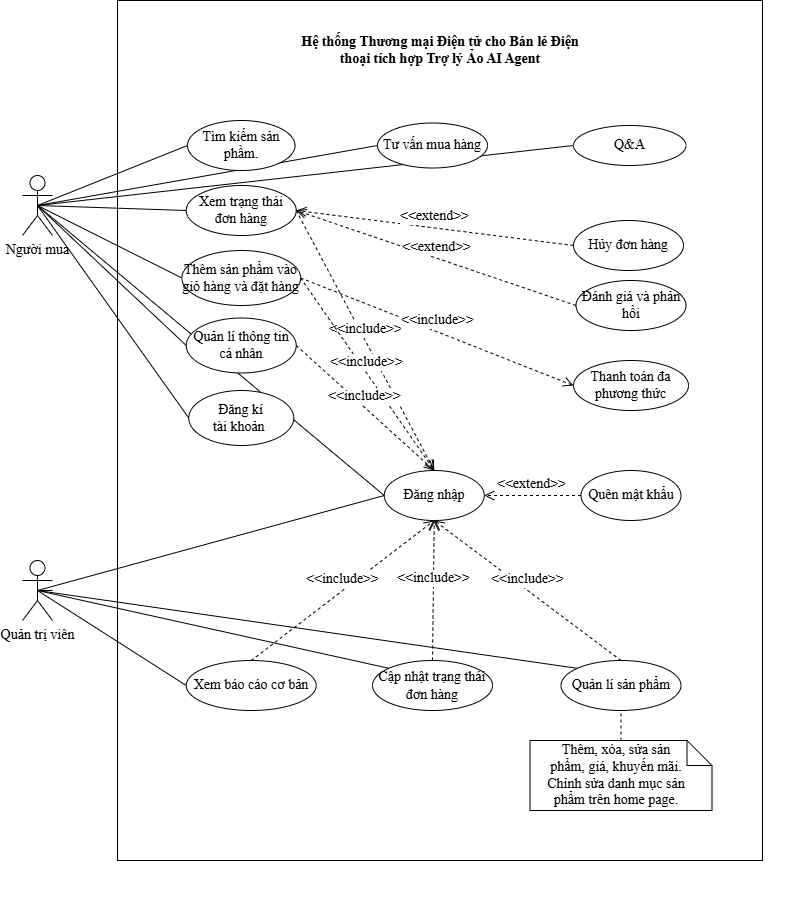
\includegraphics[width=\textwidth]{images/chap3/use_case_diagram/whole_system.png}
    % \vspace{0.5cm}
    \caption{Use case diagram tổng thể của hệ thống}
    \label{fig:use-case-diagram}
\end{figure}

\subsubsection{Bảng mô tả chi tiết các trường hợp sử dụng}

{
\fontsize{12pt}{14pt}\selectfont
\renewcommand{\arraystretch}{1.0} 
\setlength{\extrarowheight}{4pt}

\needspace{3\baselineskip}
\begin{longtable}{|>{\bfseries}p{4cm}|p{11.5cm}|}
\caption{Đặc tả use case: Đăng ký tài khoản}
\label{tab:uc-register} \\
\hline
\textbf{Tên trường hợp sử dụng} & Đăng ký tài khoản \\
\hline
\textbf{Tóm tắt mô tả} & Cho phép khách hàng tạo tài khoản mới. Tài khoản quản trị viên được cấp riêng và không thể tự đăng ký. \\
\hline
\textbf{Tác nhân} & Khách hàng \\
\hline
\textbf{Tiền điều kiện} & 1. Hệ thống hoạt động bình thường. \\
& 2. Cơ sở dữ liệu được kết nối với hệ thống. \\
& 3. Kết nối với internet được đảm bảo. \\
& 4. Khách hàng chưa có tài khoản trong hệ thống. \\
\hline
\textbf{Sự kiện kích hoạt} & Khách hàng nhấn nút “Đăng ký” trên giao diện hệ thống. \\
\hline
\textbf{Các bước thực hiện} & 1. Hệ thống hiển thị biểu mẫu đăng ký. \\
& 2. Khách hàng nhập thông tin bắt buộc (email/số điện thoại, mật khẩu,...). \\
& 3. Hệ thống kiểm tra tính hợp lệ của thông tin. \\
& 4. Hệ thống lưu thông tin khách hàng vào cơ sở dữ liệu. \\
& 5. Hệ thống xác nhận đăng ký thành công. \\
& 6. Khách hàng có thể đăng nhập sau khi xác nhận. \\
\hline
\textbf{Hậu điều kiện} & Tài khoản mới được tạo thành công và khách hàng có thể đăng nhập. \\
\hline
\textbf{Luồng thay thế} & Không. \\
\hline
\textbf{Luồng ngoại lệ} & Ngoại lệ 1: Tại bước 3 \\
& 3a. Nếu email đã tồn tại, hệ thống thông báo (\textit{yêu cầu nhập lại email khác}). \\
& 3b. Nếu mật khẩu không đạt yêu cầu, hệ thống hiển thị thông báo lỗi và yêu cầu đổi mật khẩu khác. \\
& 3c. Nếu các thông tin khác không hợp lệ hoặc chưa điền đủ các trường bắt buộc, hệ thống báo lỗi và yêu cầu nhập chính xác. \\
\hline
\end{longtable}

\needspace{3\baselineskip}
\begin{longtable}{|>{\bfseries}p{4cm}|p{11.5cm}|}
\caption{Đặc tả use case: Đăng nhập}
\label{tab:uc-login} \\
\hline
\textbf{Tên trường hợp sử dụng} & Đăng nhập \\
\hline
\textbf{Tóm tắt mô tả} & Cho phép người dùng đăng nhập vào hệ thống bằng tài khoản đã đăng ký. \\
\hline
\textbf{Tác nhân} & Khách hàng, quản trị viên \\
\hline
\textbf{Tiền điều kiện} & 1. Hệ thống hoạt động bình thường. \newline
2. Cơ sở dữ liệu được kết nối với hệ thống. \newline
3. Kết nối với internet được đảm bảo. \newline
4. Người dùng đã có tài khoản trong hệ thống.\\
\hline
\textbf{Sự kiện kích hoạt} & Người dùng nhấn nút “Đăng nhập” trên giao diện hệ thống. \\
\hline
\textbf{Các bước thực hiện} & 1. Hệ thống hiển thị màn hình đăng nhập. \newline
2. Người dùng nhập thông tin đăng nhập. \newline
3. Hệ thống xác thực thông tin đăng nhập. \newline
4. Người dùng được chuyển đến trang chủ nếu đăng nhập thành công. \\
\hline
\textbf{Hậu điều kiện} & Người dùng đã đăng nhập thành công vào hệ thống. \\
\hline
\textbf{Luồng thay thế} & \textbf{Luồng thay thế 1: Tại bước 2} \newline
2a. Đối với người dùng là khách hàng, nếu quên mật khẩu, khách hàng nhấn chọn nút “Quên mật khẩu” để chuyển đến trang cấp lại mật khẩu. \newline
2b. Đối với người dùng là khách hàng, nếu chọn phương thức đăng nhập bằng Google, hệ thống sẽ chuyển đến trang xác thực của Google\\
\hline
\textbf{Luồng ngoại lệ} & \textbf{Ngoại lệ 1: Tại bước 3} \newline
3a. Thông tin đăng nhập không hợp lệ (sai tên tài khoản hoặc mật khẩu), hệ thống hiển thị thông báo lỗi và yêu cầu người dùng thử lại. \\
\hline
\end{longtable}

\needspace{3\baselineskip}
\begin{longtable}{|>{\bfseries}p{4cm}|p{11.5cm}|}
\caption{Đặc tả use case: Quên mật khẩu}
\label{tab:uc-forgot-password} \\
\hline
\textbf{Tên trường hợp sử dụng} & Quên mật khẩu \\
\hline
\textbf{Tóm tắt mô tả} & Cho phép khách hàng lấy lại mật khẩu đã quên. \\
\hline
\textbf{Tác nhân} & Khách hàng\\
\hline
\textbf{Tiền điều kiện} & 1. Hệ thống hoạt động bình thường. \newline
2. Cơ sở dữ liệu được kết nối với hệ thống. \newline
3. Kết nối với internet được đảm bảo. \newline
4. Người dùng đã có tài khoản trong hệ thống. \\
\hline
\textbf{Sự kiện kích hoạt} & Khách hàng nhấn nút “Quên mật khẩu”. \\
\hline
\textbf{Các bước thực hiện} & 1. Hệ thống hiển thị màn hình quên mật khẩu. \newline
2. Khách hàng nhập thông tin email hoặc số điện thoại đã đăng ký tài khoản. \newline
3. Hệ thống xác thực thông tin. \newline
4. Hệ thống gửi đường dẫn đến trang đổi mật khẩu đến email hoặc sms của khách hàng. \newline
5. Khách hàng nhập mật khẩu mới. \newline
6. Hệ thống kiểm tra và cập nhật mật khẩu mới. \\
\hline
\textbf{Hậu điều kiện} & Khách hàng thiết lập mật khẩu mới thành công. \\
\hline
\textbf{Luồng thay thế} & Không \\
\hline
\textbf{Luồng ngoại lệ} & \textbf{Ngoại lệ 1: Tại bước 3} \newline
3a. Thông tin email hoặc số điện thoại không tồn tại trong hệ thống. \newline
\textbf{Ngoại lệ 2: Tại bước 6} \newline
6a. Mật khẩu mới không hợp lệ hoặc không đúng định dạng yêu cầu. \\
\hline
\end{longtable}

\needspace{3\baselineskip}
\begin{longtable}{|>{\bfseries}p{4cm}|p{11.5cm}|}
\caption{Đặc tả trường hợp sử dụng: Quản lý thông tin cá nhân}
\label{tab:uc-profile-management} \\
\hline
\textbf{Tên trường hợp sử dụng} & Quản lý thông tin cá nhân \\
\hline
\textbf{Tóm tắt mô tả} & Khách hàng xem và cập nhật thông tin cá nhân của mình trên hệ thống. \\
\hline
\textbf{Tác nhân} & Khách hàng. \\
\hline
\textbf{Tiền điều kiện} & 1. Hệ thống hoạt động bình thường. \newline
2. Cơ sở dữ liệu được kết nối với hệ thống. \newline
3. Kết nối với internet được đảm bảo. \newline
4. Khách hàng đã đăng nhập thành công vào hệ thống. \\
\hline
\textbf{Sự kiện kích hoạt} & Khách hàng truy cập vào mục “Thông tin cá nhân” trên giao diện. \\
\hline
\textbf{Các bước thực hiện} & 1. Hệ thống hiển thị thông tin cá nhân hiện tại của khách hàng. \newline
2. Khách hàng chọn chức năng chỉnh sửa thông tin. \newline
3. Khách hàng nhập các thông tin mới cần thay đổi. \newline
4. Hệ thống thực hiện kiểm tra, lưu thay đổi và cập nhật hồ sơ vào cơ sở dữ liệu. \\
\hline
\textbf{Hậu điều kiện} & Thông tin cá nhân mới được cập nhật thành công và hiển thị chính xác. \\
\hline
\textbf{Luồng thay thế} & \textbf{Luồng thay thế 1: Tại bước 2} \newline
2a. Nếu khách hàng chỉ xem lại thông tin cá nhân mà không cần chỉnh sửa thì không chọn nút chỉnh sửa thông tin cá nhân. \\
\hline
\textbf{Luồng ngoại lệ} & \textbf{Ngoại lệ 1: Tại bước 3} \newline
3a. Thông tin cập nhật không hợp lệ (sai định dạng hoặc thiếu trường bắt buộc), hệ thống thông báo lỗi. \\
\hline
\end{longtable}

\needspace{3\baselineskip}
\begin{longtable}{|>{\bfseries}p{4cm}|p{11.5cm}|}
\caption{Đặc tả trường hợp sử dụng: Tìm kiếm sản phẩm}
\label{tab:uc-search-product} \\
\hline
\textbf{Tên trường hợp sử dụng} & Tìm kiếm sản phẩm \\
\hline
\textbf{Tóm tắt mô tả} & Cho phép khách hàng tìm kiếm sản phẩm theo từ khóa hoặc các tiêu chí bộ lọc. \\
\hline
\textbf{Tác nhân} & Khách hàng. \\
\hline
\textbf{Tiền điều kiện} & 1. Hệ thống hoạt động bình thường. \newline
2. Cơ sở dữ liệu được kết nối với hệ thống. \newline
3. Kết nối với internet được đảm bảo. \\
\hline
\textbf{Sự kiện kích hoạt} & Khách hàng nhập từ khóa vào thanh tìm kiếm hoặc lựa chọn các tiêu chí lọc sản phẩm. \\
\hline
\textbf{Các bước thực hiện} & 1. Khách hàng nhập từ khóa hoặc chọn bộ lọc sản phẩm (giá, cấu hình, hãng...). \newline
2. Hệ thống thực hiện truy vấn cơ sở dữ liệu để tìm kiếm sản phẩm phù hợp. \newline
3. Hệ thống hiển thị danh sách các sản phẩm thỏa mãn điều kiện. \\
\hline
\textbf{Hậu điều kiện} & Danh sách sản phẩm hiển thị phù hợp với tiêu chí tìm kiếm của khách hàng. \\
\hline
\textbf{Luồng thay thế} & Không. \\
\hline
\textbf{Luồng ngoại lệ} & \textbf{Ngoại lệ 1: Tại bước 2} \newline
2a. Nếu xảy ra lỗi kết nối cơ sở dữ liệu, hệ thống thông báo lỗi và yêu cầu người dùng thử lại. \newline
\textbf{Ngoại lệ 2: Tại bước 3} \newline
3a. Nếu không tìm thấy sản phẩm nào phù hợp, hệ thống hiển thị thông báo "Không tìm thấy sản phẩm" kèm theo các gợi ý khác. \\
\hline
\end{longtable}

\needspace{3\baselineskip}
\begin{longtable}{|>{\bfseries}p{4cm}|p{11.5cm}|}
\caption{Đặc tả trường hợp sử dụng: Gợi ý sản phẩm}
\label{tab:uc-product-suggestion} \\
\hline
\textbf{Tên trường hợp sử dụng} & Gợi ý sản phẩm \\
\hline
\textbf{Tóm tắt mô tả} & Hệ thống AI ChatBot phân tích hành vi, lịch sử mua sắm và từ khóa tìm kiếm để đưa ra gợi ý sản phẩm cá nhân hóa. Đây là trường hợp sử dụng mở rộng từ “Tìm kiếm sản phẩm”. \\
\hline
\textbf{Tác nhân} & AI ChatBot. \\
\hline
\textbf{Tiền điều kiện} & 1. Hệ thống hoạt động bình thường. \newline
2. Cơ sở dữ liệu được kết nối với hệ thống. \newline
3. Kết nối với internet được đảm bảo. \newline
4. Trường hợp sử dụng “Tìm kiếm sản phẩm” đã được khởi động. \newline
5. Dữ liệu hành vi và lịch sử khách hàng được lưu trữ. \newline
6. AI ChatBot hoạt động và có quyền truy cập dữ liệu sản phẩm. \\
\hline
\textbf{Sự kiện kích hoạt} & Khách hàng tương tác với ChatBot. \\
\hline
\textbf{Các bước thực hiện} & 1. AI ChatBot phân tích từ khóa, lịch sử mua sắm, và hành vi duyệt web của người dùng. \newline
2. Hệ thống hiển thị câu trả lời chứa gợi ý sản phẩm phù hợp ngay trong hộp thoại chat. \\
\hline
\textbf{Hậu điều kiện} & Danh sách gợi ý sản phẩm cá nhân hóa được hiển thị thành công cho khách hàng. \\
\hline
\textbf{Luồng thay thế} & Không. \\
\hline
\textbf{Luồng ngoại lệ} & \textbf{Ngoại lệ 1: Tại bước 1} \newline
1a. Nếu xảy ra lỗi kết nối cơ sở dữ liệu hoặc dịch vụ AI, hệ thống thông báo lỗi và yêu cầu người dùng thử lại. \newline
\textbf{Ngoại lệ 2: Tại bước 2} \newline
2a. Nếu không tìm thấy sản phẩm nào phù hợp với sở thích hoặc lịch sử của người dùng, hệ thống hiển thị thông báo mặc định hoặc gợi ý các sản phẩm phổ biến nhất. \\
\hline
\end{longtable}

\needspace{3\baselineskip}
\begin{longtable}{|>{\bfseries}p{4cm}|p{11.5cm}|}
\caption{Đặc tả trường hợp sử dụng: Thêm sản phẩm vào giỏ hàng và đặt hàng}
\label{tab:uc-add-to-cart-checkout} \\
\hline
\textbf{Tên trường hợp sử dụng} & Thêm sản phẩm vào giỏ hàng và đặt hàng \\
\hline
\textbf{Tóm tắt mô tả} & Cho phép khách hàng lựa chọn sản phẩm, thêm vào giỏ hàng và thực hiện quy trình đặt hàng với nhiều phương thức thanh toán khác nhau. \\
\hline
\textbf{Tác nhân} & Khách hàng \\
\hline
\textbf{Tiền điều kiện} & 1. Hệ thống hoạt động bình thường. \newline
2. Cơ sở dữ liệu được kết nối với hệ thống. \newline
3. Kết nối với internet được đảm bảo. \newline
4. Sản phẩm còn hàng trong kho. \\
\hline
\textbf{Sự kiện kích hoạt} & Khách hàng chọn sản phẩm và nhấn nút “Thêm vào giỏ hàng” hoặc “Đặt hàng”. \\
\hline
\textbf{Các bước thực hiện} & 1. Khách hàng chọn sản phẩm cần mua. \newline
2. Hệ thống hiển thị chi tiết sản phẩm và nút “Thêm vào giỏ hàng”. \newline
3. Khách hàng thêm sản phẩm vào giỏ. \newline
4. Hệ thống cập nhật giỏ hàng và hiển thị tổng số lượng, giá tiền. \newline
5. Khách hàng chọn “Đặt hàng”. \newline
6. Hệ thống yêu cầu khách hàng xác nhận địa chỉ giao hàng, phương thức thanh toán. \newline
7. Hệ thống kiểm tra tính hợp lệ của thông tin và số lượng tồn kho. \newline
8. Hệ thống tạo đơn hàng và gửi xác nhận cho khách hàng. \\
\hline
\textbf{Hậu điều kiện} & Đơn hàng được tạo thành công và lưu trong hệ thống, khách hàng nhận thông báo xác nhận. \\
\hline
\textbf{Luồng thay thế} & \textbf{Luồng thay thế 1: Tại bước 4} \newline
4a. Khách hàng không đặt hàng ngay mà chỉ thêm sản phẩm vào giỏ hàng và tiếp tục mua sắm. \\
\hline
\textbf{Luồng ngoại lệ} & \textbf{Ngoại lệ 1: Tại bước 6} \newline
6a. Nếu phương thức thanh toán hiện tại không hỗ trợ hoặc xảy ra lỗi cổng thanh toán, hệ thống báo lỗi và yêu cầu khách hàng chọn phương thức thanh toán khác. \\
\hline
\end{longtable}

\needspace{3\baselineskip}
\begin{longtable}{|>{\bfseries}p{4cm}|p{11.5cm}|}
\caption{Đặc tả trường hợp sử dụng: Hỗ trợ đặt hàng}
\label{tab:uc-chatbot-order-support} \\
\hline
\textbf{Tên trường hợp sử dụng} & Hỗ trợ đặt hàng \\
\hline
\textbf{Tóm tắt mô tả} & AI ChatBot dựa vào tin nhắn của khách hàng từ đó xác định nhu cầu và gửi đề xuất đặt hàng trực tiếp cho khách hàng trong cửa sổ trò chuyện. \\
\hline
\textbf{Tác nhân} & AI ChatBot. \\
\hline
\textbf{Tiền điều kiện} & 1. Hệ thống hoạt động bình thường. \newline
2. Cơ sở dữ liệu được kết nối với hệ thống. \newline
3. Kết nối với internet được đảm bảo. \newline
4. Trường hợp sử dụng “Thêm sản phẩm vào giỏ hàng và đặt hàng” đã được khởi động. \newline
5. AI ChatBot hoạt động bình thường và được tích hợp vào hệ thống. \newline
6. Dữ liệu sản phẩm và lịch sử khách hàng khả dụng để phân tích. \\
\hline
\textbf{Sự kiện kích hoạt} & Khách hàng trò chuyện với AI ChatBot và có yêu cầu liên quan đến việc đặt hàng. \\
\hline
\textbf{Các bước thực hiện} & 1. Khách hàng gửi các tin nhắn về nhu cầu đặt hàng để AI có đủ thông tin về đơn hàng. \newline
2. AI ChatBot tổng hợp thông tin về đơn hàng và hiển thị cửa sổ hoặc nút xác nhận đặt hàng. \newline
3. Khách hàng có thể chọn “Đồng ý” để tiến hành đặt hàng hoặc “Không đồng ý” để từ chối. \newline
4. Nếu khách hàng đồng ý, hệ thống tiếp tục các bước trong quy trình đặt hàng chính thức. \\
\hline
\textbf{Hậu điều kiện} & Nếu khách hàng đồng ý, đơn hàng được xác nhận và hệ thống chuyển sang quy trình đặt hàng. Ngược lại, không có đơn hàng nào được tạo. Hệ thống lưu lại lịch sử tương tác để cải thiện gợi ý. \\
\hline
\textbf{Luồng thay thế} & Không. \\
\hline
\textbf{Luồng ngoại lệ} & \textbf{Ngoại lệ 1: Tại bước 2} \newline
2a. Nếu xảy ra các lỗi về kết nối hoặc truy xuất dữ liệu sản phẩm, hệ thống thông báo lỗi và yêu cầu người dùng thử lại. \\
\hline
\end{longtable}

\needspace{3\baselineskip}
\begin{longtable}{|>{\bfseries}p{4cm}|p{11.5cm}|}
\caption{Đặc tả trường hợp sử dụng: Thanh toán đa phương thức}
\label{tab:uc-multipayment} \\
\hline
\textbf{Tên trường hợp sử dụng} & Thanh toán đa phương thức \\
\hline
\textbf{Tóm tắt mô tả} & Cho phép khách hàng thanh toán đơn hàng bằng nhiều phương thức khác nhau như: tiền mặt khi nhận hàng (COD), thẻ ngân hàng, ví điện tử, hoặc các cổng thanh toán trực tuyến. \\
\hline
\textbf{Tác nhân} & Khách hàng. \\
\hline
\textbf{Tiền điều kiện} & 1. Hệ thống hoạt động bình thường. \newline
2. Cơ sở dữ liệu được kết nối với hệ thống. \newline
3. Kết nối với Internet được đảm bảo. \newline
4. Đơn hàng đã được tạo thành công. \newline
5. Hệ thống kết nối thành công với các cổng thanh toán bên thứ ba (nếu có). \\
\hline
\textbf{Sự kiện kích hoạt} & Khách hàng nhấn chọn “Thanh toán” sau khi xác nhận đơn hàng đối với các phương thức trả trước. \\
\hline
\textbf{Các bước thực hiện} & 1. Tùy vào phương thức thanh toán mà khách hàng chọn, hệ thống sẽ hiển thị biểu mẫu hoặc trang thanh toán tương ứng. \newline
2. Khách hàng thực hiện các thao tác thanh toán theo hướng dẫn. \newline
3. Hệ thống hiển thị trạng thái giao dịch và cập nhật trạng thái đơn hàng tương ứng. \\
\hline
\textbf{Hậu điều kiện} & Thanh toán được xử lý thành công và thông tin giao dịch được lưu trữ chính xác trong hệ thống. \\
\hline
\textbf{Luồng thay thế} & \textbf{Luồng thay thế 1: Tại bước 2} \newline
2a. Nếu phương thức thanh toán là “Thanh toán khi nhận hàng” (COD), khách hàng bỏ qua bước thanh toán trực tuyến, hệ thống tự động cập nhật trạng thái đơn hàng sang “Chờ giao hàng”. \\
\hline
\textbf{Luồng ngoại lệ} & \textbf{Ngoại lệ 1: Tại bước 2} \newline
2a. Giao dịch thất bại (sai mã OTP, số dư không đủ...), hệ thống thông báo lỗi và yêu cầu người dùng thử lại hoặc chọn phương thức khác. \newline
2b. Lỗi kết nối với cổng thanh toán bên thứ ba, hệ thống hiển thị thông báo sự cố và giữ đơn hàng ở trạng thái “Chờ thanh toán”. \\
\hline
\end{longtable}

\needspace{3\baselineskip}
\begin{longtable}{|>{\bfseries}p{4cm}|p{11.5cm}|}
\caption{Đặc tả trường hợp sử dụng: Hủy đơn hàng}
\label{tab:uc-cancel-order} \\
\hline
\textbf{Tên trường hợp sử dụng} & Hủy đơn hàng \\
\hline
\textbf{Tóm tắt mô tả} & Cho phép khách hàng hủy đơn hàng đã đặt trong một số điều kiện nhất định. \\
\hline
\textbf{Tác nhân} & Khách hàng. \\
\hline
\textbf{Tiền điều kiện} & 1. Hệ thống hoạt động bình thường. \newline
2. Cơ sở dữ liệu được kết nối với hệ thống. \newline
3. Kết nối với Internet được đảm bảo. \newline
4. Đơn hàng đang ở trạng thái cho phép hủy (ví dụ: Chờ xác nhận hoặc Chờ lấy hàng). \\
\hline
\textbf{Sự kiện kích hoạt} & Khách hàng nhấn chọn chức năng hủy đơn hàng. \\
\hline
\textbf{Các bước thực hiện} & 1. Khách hàng mở danh sách đơn hàng cá nhân và chọn đơn hàng muốn hủy. \newline
2. Hệ thống hiển thị thông tin chi tiết của đơn hàng đó. \newline
3. Khách hàng nhấn nút “Hủy đơn hàng”. \newline
4. Hệ thống yêu cầu khách hàng xác nhận lại và chọn/nhập lý do hủy. \newline
5. Hệ thống thực hiện kiểm tra các điều kiện ràng buộc để hủy đơn hàng. \newline
6. Hệ thống cập nhật trạng thái đơn hàng thành “Đã hủy” và gửi thông báo xác nhận cho khách hàng. \\
\hline
\textbf{Hậu điều kiện} & Đơn hàng được chuyển sang trạng thái hủy thành công và hệ thống ngừng các quy trình xử lý tiếp theo. \\
\hline
\textbf{Luồng thay thế} & \textbf{Luồng thay thế 1: Tại bước 4} \newline
4a. Khách hàng thay đổi ý định và từ chối xác nhận hủy, hệ thống đóng cửa sổ xác nhận và giữ nguyên trạng thái hiện tại của đơn hàng. \\
\hline
\textbf{Luồng ngoại lệ} & \textbf{Ngoại lệ 1: Tại bước 5} \newline
5a. Đơn hàng đã chuyển sang trạng thái không thể hủy (ví dụ: Đang giao hàng), hệ thống thông báo từ chối yêu cầu hủy đơn hàng. \newline
5b. Lỗi kết nối cơ sở dữ liệu hoặc hệ thống không phản hồi, thông báo lỗi cho người dùng và không thay đổi trạng thái đơn hàng. \\
\hline
\end{longtable}

\needspace{3\baselineskip}
\begin{longtable}{|>{\bfseries}p{4cm}|p{11.5cm}|}
\caption{Đặc tả trường hợp sử dụng: Hỗ trợ hủy đơn hàng}
\label{tab:uc-chatbot-cancel-support} \\
\hline
\textbf{Tên trường hợp sử dụng} & Hỗ trợ hủy đơn hàng \\
\hline
\textbf{Tóm tắt mô tả} & AI ChatBot hỗ trợ khách hàng thực hiện các thao tác hủy đơn hàng nếu họ gặp khó khăn trong quá trình sử dụng giao diện thông thường. Đây là trường hợp sử dụng mở rộng từ “Hủy đơn hàng”. \\
\hline
\textbf{Tác nhân} & AI ChatBot \\
\hline
\textbf{Tiền điều kiện} & 1. Hệ thống hoạt động bình thường. \newline
2. Cơ sở dữ liệu được kết nối với hệ thống. \newline
3. Kết nối với Internet được đảm bảo. \newline
4. Trường hợp sử dụng “Hủy đơn hàng” đã được khởi động. \newline
5. AI ChatBot ở trạng thái sẵn sàng phục vụ. \newline
6. Đơn hàng hiện đang ở trạng thái cho phép hủy. \\
\hline
\textbf{Sự kiện kích hoạt} & Khách hàng gửi yêu cầu trợ giúp khi muốn thực hiện hủy đơn hàng thông qua khung trò chuyện. \\
\hline
\textbf{Các bước thực hiện} & 1. Khách hàng gửi tin nhắn yêu cầu hủy đơn hàng cho AI ChatBot. \newline
2. AI ChatBot truy xuất, hiển thị thông tin đơn hàng tương ứng và yêu cầu khách hàng xác nhận lại. \newline
3. Khách hàng thực hiện xác nhận đồng ý hủy đơn hàng. \newline
4. Hệ thống tiến hành kiểm tra các điều kiện ràng buộc về trạng thái đơn hàng. \newline
5. Nếu mọi điều kiện hợp lệ, hệ thống tự động cập nhật trạng thái đơn hàng thành “Đã hủy”. \newline
6. AI ChatBot gửi thông báo kết quả hủy đơn hàng thành công cho khách hàng. \\
\hline
\textbf{Hậu điều kiện} & Đơn hàng được chuyển sang trạng thái hủy thành công thông qua tương tác với AI ChatBot. \\
\hline
\textbf{Luồng thay thế} & \textbf{Luồng thay thế 1: Tại bước 3} \newline
3a. Khách hàng thay đổi ý định và từ chối xác nhận lại tại bước 3, hệ thống giữ nguyên trạng thái đơn hàng. \\
\hline
\textbf{Luồng ngoại lệ} & \textbf{Ngoại lệ 1: Tại bước 5} \newline
5a. Đơn hàng đã chuyển sang trạng thái không còn được phép hủy (v.d: Đang vận chuyển), hệ thống thông báo nguyên nhân đơn hàng không thể hủy. \newline
5b. Xảy ra lỗi kết nối cơ sở dữ liệu, hệ thống hiển thị thông báo sự cố kỹ thuật và giữ nguyên trạng thái đơn hàng. \\
\hline
\end{longtable}

\needspace{3\baselineskip}
\begin{longtable}{|>{\bfseries}p{4cm}|p{11.5cm}|}
\caption{Đặc tả trường hợp sử dụng: Xem trạng thái đơn hàng}
\label{tab:uc-view-order-status} \\
\hline
\textbf{Tên trường hợp sử dụng} & Xem trạng thái đơn hàng \\
\hline
\textbf{Tóm tắt mô tả} & Cho phép khách hàng theo dõi tiến trình của các đơn hàng sau khi đặt (chờ xác nhận, đang giao, đã giao thành công hoặc đã hủy). \\
\hline
\textbf{Tác nhân} & Khách hàng \\
\hline
\textbf{Tiền điều kiện} & 1. Hệ thống hoạt động bình thường. \newline
2. Cơ sở dữ liệu được kết nối với hệ thống. \newline
3. Kết nối với Internet được đảm bảo. \newline
4. Khách hàng đã đăng nhập thành công vào hệ thống. \\
\hline
\textbf{Sự kiện kích hoạt} & Khách hàng chọn chức năng “Đơn hàng của tôi” hoặc “Xem đơn hàng” trên giao diện người dùng. \\
\hline
\textbf{Các bước thực hiện} & 1. Khách hàng truy cập vào mục danh sách đơn hàng theo trạng thái cần xem. \newline
2. Hệ thống truy xuất và hiển thị danh sách các đơn hàng gần nhất phù hợp với yêu cầu. \newline
3. Khách hàng chọn một đơn hàng cụ thể để xem chi tiết. \newline
4. Hệ thống hiển thị chi tiết trạng thái, lộ trình và tiến trình xử lý hiện tại của đơn hàng đó. \\
\hline
\textbf{Hậu điều kiện} & Khách hàng nắm bắt được thông tin chi tiết về trạng thái và tiến trình xử lý thực tế của đơn hàng. \\
\hline
\textbf{Luồng thay thế} & Không. \\
\hline
\textbf{Luồng ngoại lệ} & \textbf{Ngoại lệ 1: Tại bước 2} \newline
2a. Nếu không có đơn hàng nào phù hợp với bộ lọc hoặc lịch sử, hệ thống hiển thị danh sách trống và thông báo cho người dùng. \\
\hline
\end{longtable}

\needspace{3\baselineskip}
\begin{longtable}{|>{\bfseries}p{4cm}|p{11.5cm}|}
\caption{Đặc tả trường hợp sử dụng: Hỗ trợ trong và sau mua hàng}
\label{tab:uc-post-purchase-support} \\
\hline
\textbf{Tên trường hợp sử dụng} & Hỗ trợ trong và sau mua hàng \\
\hline
\textbf{Tóm tắt mô tả} & AI ChatBot cung cấp thông tin, tư vấn và giải đáp thắc mắc liên quan đến đơn hàng trong quá trình xử lý hoặc sau khi đã hoàn tất. Đây là trường hợp sử dụng mở rộng từ “Xem trạng thái đơn hàng”. \\
\hline
\textbf{Tác nhân} & AI ChatBot. \\
\hline
\textbf{Tiền điều kiện} & 1. Hệ thống hoạt động bình thường. \newline
2. Cơ sở dữ liệu được kết nối với hệ thống. \newline
3. Kết nối với Internet được đảm bảo. \newline
4. Trường hợp sử dụng “Xem trạng thái đơn hàng” đã được khởi động. \newline
5. AI ChatBot ở trạng thái sẵn sàng phục vụ. \newline
6. Dữ liệu đơn hàng và lịch sử tương tác được lưu trữ đầy đủ trong hệ thống. \\
\hline
\textbf{Sự kiện kích hoạt} & Khách hàng yêu cầu Chatbot hỗ trợ khi đang xem thông tin chi tiết của một đơn hàng. \\
\hline
\textbf{Các bước thực hiện} & 1. Khách hàng nhấn chọn nút “Trợ giúp” hoặc gửi tin nhắn trực tiếp trong giao diện ChatBot. \newline
2. AI ChatBot phân tích nội dung yêu cầu và đưa ra phản hồi tư vấn tự động dựa trên dữ liệu đơn hàng. \\
\hline
\textbf{Hậu điều kiện} & Khách hàng nhận được thông tin hỗ trợ hoặc giải pháp phù hợp cho các vấn đề liên quan đến đơn hàng. \\
\hline
\textbf{Luồng thay thế} & \textbf{Luồng thay thế 1: Tại bước 2} \newline
2a. Nếu khách hàng cần tham khảo các câu hỏi thường gặp (FAQ), AI ChatBot cung cấp liên kết trực tiếp đến trang hướng dẫn hoặc chính sách tương ứng. \\
\hline
\textbf{Luồng ngoại lệ} & \textbf{Ngoại lệ 1: Tại bước 2} \newline
2a. Nếu ChatBot không sẵn dụng hoặc xảy ra lỗi kết nối dịch vụ AI, hệ thống thông báo lỗi và cung cấp phương thức gửi yêu cầu hỗ trợ qua email cho khách hàng. \\
\hline
\end{longtable}

\needspace{3\baselineskip}
\begin{longtable}{|>{\bfseries}p{4cm}|p{11.5cm}|}
\caption{Đặc tả trường hợp sử dụng: Đánh giá và phản hồi của khách hàng}
\label{tab:uc-customer-review} \\
\hline
\textbf{Tên trường hợp sử dụng} & Đánh giá và phản hồi của khách hàng \\
\hline
\textbf{Tóm tắt mô tả} & Khách hàng có thể gửi đánh giá (số sao, nhận xét) về sản phẩm hoặc dịch vụ sau khi nhận hàng để giúp doanh nghiệp cải thiện chất lượng phục vụ. \\
\hline
\textbf{Tác nhân} & Khách hàng. \\
\hline
\textbf{Tiền điều kiện} & 1. Hệ thống hoạt động bình thường. \newline
2. Cơ sở dữ liệu được kết nối với hệ thống. \newline
3. Kết nối với Internet được đảm bảo. \newline
4. Khách hàng đã đăng nhập thành công vào hệ thống. \\
\hline
\textbf{Sự kiện kích hoạt} & Khách hàng nhấn chọn chức năng “Đánh giá” hoặc “Phản hồi” tại danh mục các đơn hàng đã giao thành công. \\
\hline
\textbf{Các bước thực hiện} & 1. Hệ thống hiển thị biểu mẫu đánh giá sản phẩm tương ứng với đơn hàng. \newline
2. Khách hàng thực hiện chọn số sao đánh giá và nhập nội dung nhận xét hoặc góp ý. \newline
3. Hệ thống kiểm tra, thực hiện lưu phản hồi vào cơ sở dữ liệu và gửi thông báo xác nhận thành công. \\
\hline
\textbf{Hậu điều kiện} & Nội dung đánh giá và phản hồi được lưu trữ trong hệ thống và sẵn sàng để hiển thị hoặc phục vụ mục đích báo cáo nội bộ. \\
\hline
\textbf{Luồng thay thế} & \textbf{Luồng thay thế 1: Tại bước 1} \newline
1a. Nếu khách hàng bỏ qua bước đánh giá và thoát màn hình, đơn hàng vẫn được giữ nguyên trạng thái hoàn tất nhưng không có dữ liệu phản hồi kèm theo. \\
\hline
\textbf{Luồng ngoại lệ} & Không. \\
\hline
\end{longtable}

\needspace{3\baselineskip}
\begin{longtable}{|>{\bfseries}p{4cm}|p{11.5cm}|}
\caption{Đặc tả trường hợp sử dụng: Quản lý sản phẩm}
\label{tab:uc-admin-product-management} \\
\hline
\textbf{Tên trường hợp sử dụng} & Quản lý sản phẩm \\
\hline
\textbf{Tóm tắt mô tả} & Cho phép quản trị viên thêm mới, chỉnh sửa thông tin, hoặc xóa sản phẩm trong danh mục hệ thống. \\
\hline
\textbf{Tác nhân} & Quản trị viên. \\
\hline
\textbf{Tiền điều kiện} & 1. Hệ thống hoạt động bình thường. \newline
2. Cơ sở dữ liệu được kết nối với hệ thống. \newline
3. Kết nối với Internet được đảm bảo. \newline
4. Quản trị viên đã đăng nhập thành công vào hệ thống quản trị. \\
\hline
\textbf{Sự kiện kích hoạt} & Quản trị viên nhấn chọn chức năng “Quản lý sản phẩm” trên giao diện quản trị điều hành. \\
\hline
\textbf{Các bước thực hiện} & 1. Quản trị viên lựa chọn tác vụ cần thực hiện: thêm mới, chỉnh sửa hoặc xóa sản phẩm. \newline
2. Hệ thống hiển thị biểu mẫu hoặc cửa sổ xác nhận tương ứng với tác vụ đã chọn. \newline
3. Quản trị viên thực hiện nhập mới hoặc cập nhật các thông tin sản phẩm. \newline
4. Hệ thống thực hiện kiểm tra tính hợp lệ của dữ liệu đầu vào. \newline
5. Hệ thống thực hiện lưu thông tin sản phẩm vào cơ sở dữ liệu. \newline
6. Hệ thống gửi thông báo xác nhận thao tác thành công cho quản trị viên. \\
\hline
\textbf{Hậu điều kiện} & Danh mục sản phẩm được cập nhật chính xác trong hệ thống và hiển thị lên giao diện người dùng. \\
\hline
\textbf{Luồng thay thế} & \textbf{Luồng thay thế 1: Tại bước 3} \newline
3a. Quản trị viên nhấn nút hủy thao tác hoặc thoát màn hình trước khi nhấn lưu, hệ thống sẽ không thực hiện bất kỳ thay đổi nào đối với dữ liệu. \\
\hline
\textbf{Luồng ngoại lệ} & \textbf{Ngoại lệ 1: Tại bước 4} \newline
4a. Nếu dữ liệu nhập vào không hợp lệ (sai định dạng giá, thiếu thông tin bắt buộc...), hệ thống báo lỗi chi tiết và yêu cầu quản trị viên hiệu chỉnh lại. \\
\hline
\end{longtable}

\needspace{3\baselineskip}
\begin{longtable}{|>{\bfseries}p{4cm}|p{11.5cm}|}
\caption{Đặc tả trường hợp sử dụng: Cập nhật trạng thái đơn hàng}
\label{tab:uc-admin-update-order-status} \\
\hline
\textbf{Tên trường hợp sử dụng} & Cập nhật trạng thái đơn hàng \\
\hline
\textbf{Tóm tắt mô tả} & Cho phép quản trị viên hoặc nhân viên vận hành thay đổi trạng thái đơn hàng (xác nhận, đang giao, đã giao, hủy) để khách hàng tiện theo dõi. \\
\hline
\textbf{Tác nhân} & Quản trị viên. \\
\hline
\textbf{Tiền điều kiện} & 1. Hệ thống hoạt động bình thường. \newline
2. Cơ sở dữ liệu được kết nối với hệ thống. \newline
3. Kết nối với Internet được đảm bảo. \newline
4. Quản trị viên đã đăng nhập thành công vào hệ thống quản trị. \\
\hline
\textbf{Sự kiện kích hoạt} & Quản trị viên chọn một đơn hàng cụ thể từ danh sách đơn hàng để thực hiện cập nhật trạng thái. \\
\hline
\textbf{Các bước thực hiện} & 1. Quản trị viên truy cập vào danh mục quản lý danh sách đơn hàng. \newline
2. Hệ thống truy xuất và hiển thị thông tin chi tiết của đơn hàng được chọn. \newline
3. Quản trị viên lựa chọn trạng thái mới phù hợp với tiến độ thực tế. \newline
4. Hệ thống thực hiện cập nhật trạng thái đơn hàng vào cơ sở dữ liệu. \newline
5. Hệ thống tự động gửi thông báo cập nhật cho khách hàng về trạng thái mới của đơn hàng. \\
\hline
\textbf{Hậu điều kiện} & Trạng thái đơn hàng được cập nhật thành công trong hệ thống và đồng bộ với giao diện của khách hàng. \\
\hline
\textbf{Luồng thay thế} & Không. \\
\hline
\textbf{Luồng ngoại lệ} & \textbf{Ngoại lệ 1: Tại bước 3} \newline
3a. Nếu đơn hàng đã bị khách hàng hủy ngay tại thời điểm quản trị viên đang thao tác cập nhật, hệ thống sẽ hiển thị thông báo lỗi và yêu cầu tải lại trang. \\
\hline
\end{longtable}

\needspace{3\baselineskip}
\begin{longtable}{|>{\bfseries}p{4cm}|p{11.5cm}|}
\caption{Đặc tả trường hợp sử dụng: Xem báo cáo cơ bản}
\label{tab:uc-admin-basic-reports} \\
\hline
\textbf{Tên trường hợp sử dụng} & Xem báo cáo cơ bản \\
\hline
\textbf{Tóm tắt mô tả} & Cho phép quản trị viên xem báo cáo tổng hợp về doanh thu, số lượng đơn hàng, các sản phẩm bán chạy và phản hồi từ phía khách hàng. \\
\hline
\textbf{Tác nhân} & Quản trị viên. \\
\hline
\textbf{Tiền điều kiện} & 1. Hệ thống hoạt động bình thường. \newline
2. Cơ sở dữ liệu được kết nối với hệ thống. \newline
3. Kết nối với Internet được đảm bảo. \newline
4. Quản trị viên đã đăng nhập thành công vào hệ thống quản trị. \\
\hline
\textbf{Sự kiện kích hoạt} & Quản trị viên nhấn chọn chức năng “Xem báo cáo” hoặc “Thống kê” từ menu điều hướng quản trị. \\
\hline
\textbf{Các bước thực hiện} & 1. Quản trị viên truy cập vào mục quản lý báo cáo và thống kê. \newline
2. Hệ thống hiển thị danh sách các loại báo cáo hiện có (doanh thu theo ngày/tháng, sản phẩm bán chạy, tổng hợp phản hồi khách hàng). \newline
3. Quản trị viên chọn loại báo cáo và các tiêu chí lọc (thời gian, danh mục) cần xem. \newline
4. Hệ thống truy xuất dữ liệu và hiển thị báo cáo dưới dạng bảng số liệu hoặc biểu đồ trực quan. \newline
5. Quản trị viên có thể chọn chức năng xuất báo cáo dưới định dạng PDF hoặc Excel để lưu trữ. \\
\hline
\textbf{Hậu điều kiện} & Quản trị viên nắm bắt được dữ liệu thống kê phục vụ cho việc phân tích kinh doanh và quản lý. \\
\hline
\textbf{Luồng thay thế} & \textbf{Luồng thay thế 1: Tại bước 3} \newline
3a. Quản trị viên thay đổi bộ lọc hoặc tiêu chí thời gian, hệ thống tự động cập nhật lại số liệu báo cáo tương ứng. \\
\hline
\textbf{Luồng ngoại lệ} & \textbf{Ngoại lệ 1: Tại bước 4} \newline
4a. Không có dữ liệu trong khoảng thời gian được chọn, hệ thống hiển thị thông báo “Không có dữ liệu phù hợp”. \newline
4b. Nếu xảy ra lỗi truy xuất dữ liệu từ máy chủ, hệ thống hiển thị thông báo lỗi kỹ thuật. \\
\hline
\end{longtable}

\setlength{\extrarowheight}{0pt} 

}